\section{Counting Sort} \label{cap:2:section:csort}

\subsection{Introdução}

O \textit{Counting} Sort é um algoritmo de ordenação bastante eficiente dada a uma quantidade de
memória equivalente as necessidades. Seu funcionamento é baseado num método de contagem, iterando pelo vetor 
origem e contando as aparições dos elementos num vetor auxiliar $K$.

Uma das características desse algoritmo é, como será apresentado, seu tempo de execução linear mas
sua grande utilização de memória a depender da necessidade. Sendo, seu uso de memória a equação \ref{cap:2:eq:countingSort:0}.

\begin{equation} \label{cap:2:eq:countingSort:0}
    M(n) = n + k \ para \ k = |\min n| + |\max n|
\end{equation}

\subsection{Implementação}

Para o algoritmo de ordenação por contagem, o pseudo-código utilizado para desenvolver o
algoritmo pode ser observado em \ref{countingSortP} retirado do livro \cite{cormen2022algorithms}.

\begin{pseudocode}[caption={Algoritmo de ordenação por contagem}, label={countingSortP}]
COUNTING-SORT(A, n, K)
let B[1:n] and C[0:K] be new arrays
for i $\gets$ 0 to k
    C[i] $\gets$ 0
for j $\gets$ 1 to n
    C[A[j]] $\gets$ C[A[j]] + 1
for i $\gets$ 1 to k
    C[i] = C[i] + C[i - 1]
for j $\gets$ n downto 1
    B[C[A[j]]] $\gets$ A[j]
    C[A[j]] $\gets$ C[A[j]] - 1
return B
\end{pseudocode}

Esse pseudo-código foi implementado na linguagem de programação C 
e pode ser observado no código seguinte:

\begin{lstlisting}[style=CStyle]
void cSort(unsigned char * v, int n)
{
    int i, j;

    int size = __UINT8_MAX__;

    unsigned char B[n];
    int C[size + 1];

    for (i = 0; i < size + 1; i++)
    {
        C[i] = 0;
    }

    for (j = 0; j < n; j++)
    {
        C[v[j]]++;
    }

    for (i = 1; i <= size; i++)
    {
        C[i] = C[i] + C[i - 1];
    }

    for (j = n - 1; j >= 0; j--)
    {
        B[C[v[j]] - 1] = v[j];
        C[v[j]]--;
    }

    for (i = 0; i < n; i++)
    {
        v[i] = B[i];
    }

}
\end{lstlisting}
        

Essa implementação do algoritmo em C, leva em consideração que o vetor
a ser ordenado é de caracteres, portanto, o vetor auxiliar $K$ sempre será
igual a 256, por ser o máximo possível de distância entre o mínimo e o 
máximo do vetor origem.

\subsection{Análise do algoritmo e notação assintótica}

Para que seja determinada a razão de crescimento do algoritmo de ordenação por contagem, é necessário
perceber os tempos de execução de cada linha do pseudo-código \ref{countingSortP}.
Nesse caso, pode-se ter como base a equação \ref{cap:2:eq:countingSort:1}.

\begin{equation} \label{cap:2:eq:countingSort:1}
    T(n) = C_2 + C_{14} + \sum_{i=1}^{n}(C_5 + C_{12} + C_{13}) + \sum_{i=1}^{k}(C_3 + C_8)
\end{equation}

Podemos assumir a relação entre a equação 
\ref{cap:2:eq:countingSort:1} com a equação \ref{cap:2:eq:countingSort:2}.

\begin{equation} \label{cap:2:eq:countingSort:2}
    T(n) = an + bk + c\  para\  a = (C_5 + C_{12} + C_{13}) \ ,b = (C_3 + C_8) \ e \ c = (C_1 + C_{14})
\end{equation}

Com isso, pode-se determinar as seguintes notações assintóticas para o algoritmo de ordenação por contagem:

\begin{align*} \label{cap:2:eq:countingSort:3}
    O(n) &= n + k \\ 
    \Omega(n) &= n + k \\
    \Theta(n) &= n + k
\end{align*}

\subsection{Comparação teórica-prática}

Para melhor compreensão do tempo de execução do algoritmo de ordenação por contagem, pode-se observar o gráfico 
\ref{cap:2:graph:countingSort} que apresentam o tempo de execução para o algoritmo de ordenação por contagem
para 8192 casos diferentes com o número de entradas $n$ variando de 1 a 1048576.

\begin{figure}[h]
    \centering
    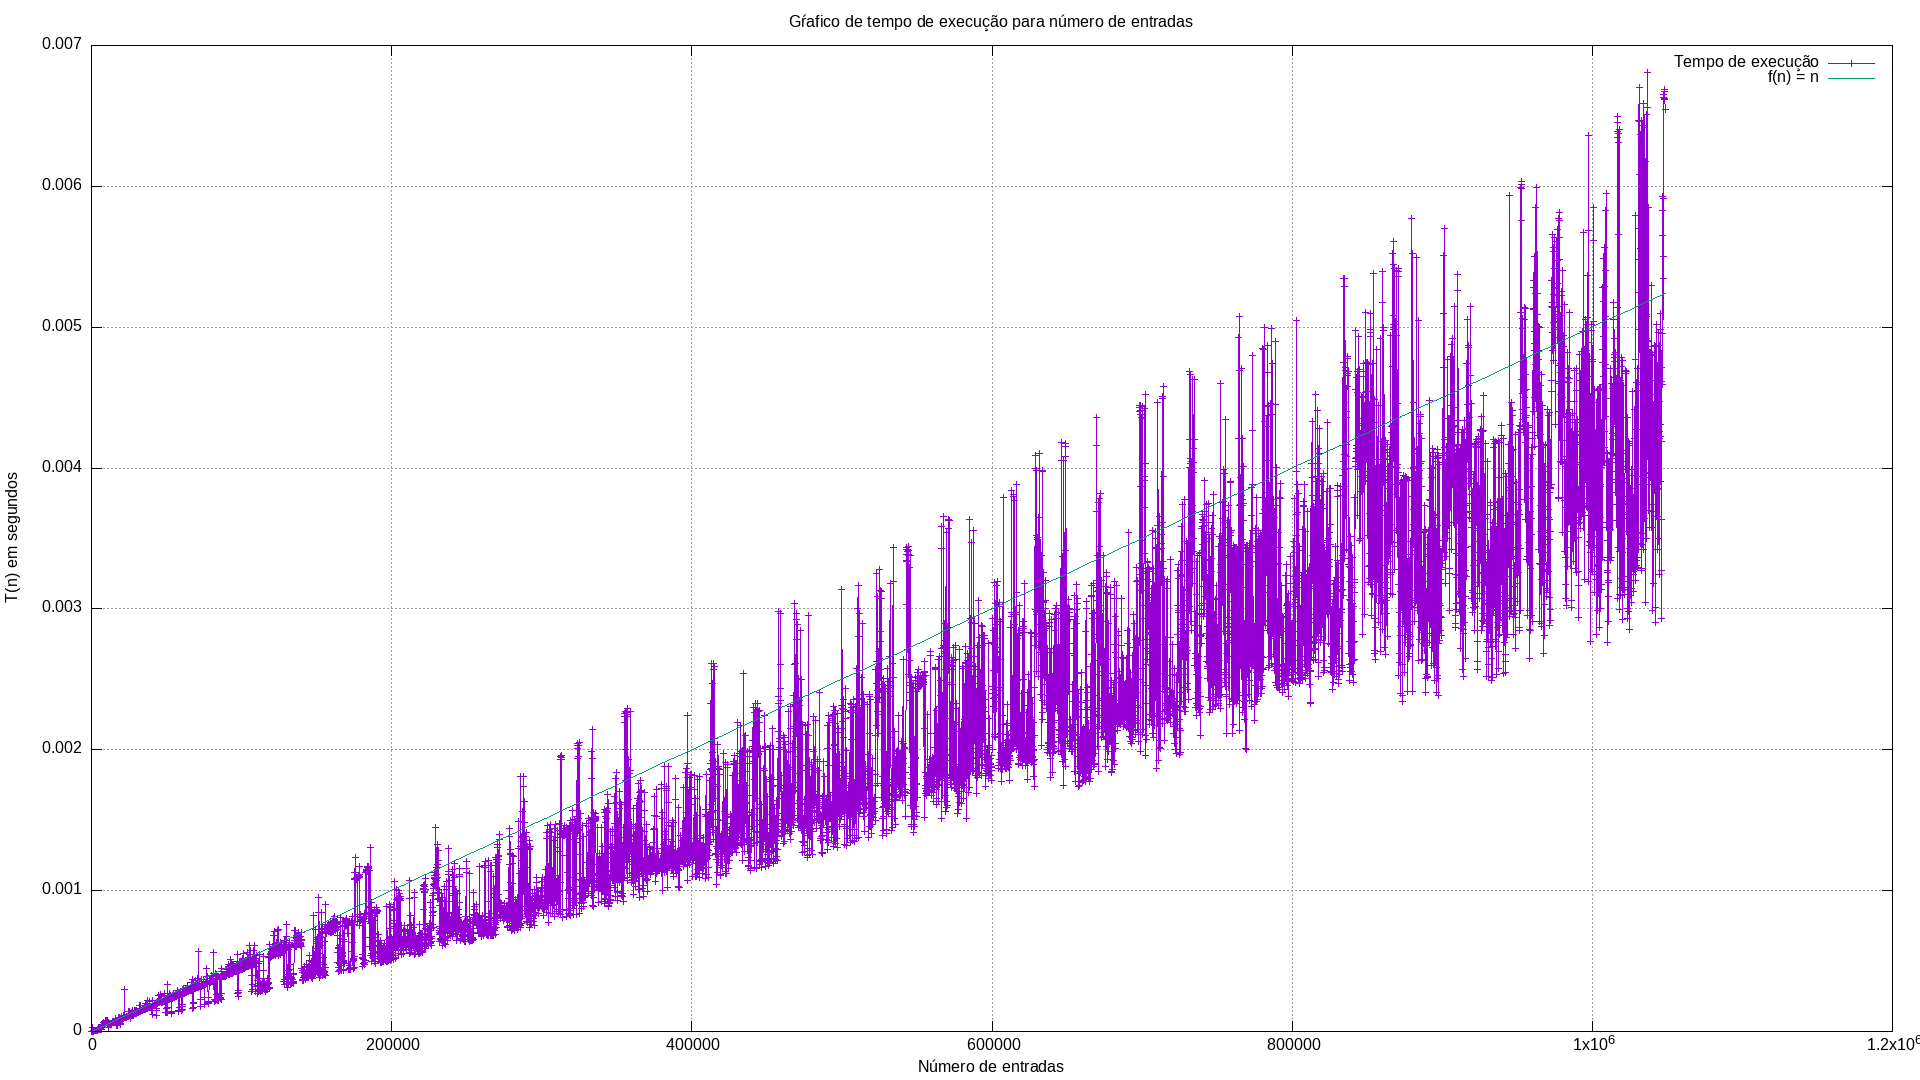
\includegraphics[width=\textwidth]{image/graphics/countingSort.png}
    \caption{Gráfico com tempo de execução do algoritmo de ordenação por contagem}
    \label{cap:2:graph:countingSort}
\end{figure}

No gráfico \ref{cap:2:graph:countingSort}, é possível perceber que o tempo de execução do algoritmo se aproxima
da função $f(n)$ que é uma função linear para $n$ com uma redução de escala para melhor percepção e comparação. Então,
utilizando como base o gráfico \ref{cap:2:graph:countingSort}, pode-se confirmar que a ordem de crescimento determinada é
precisa.

\subsection{Discussão sobre tempo de execução e uso de memória}

Sobre seu tempo de execução, o algoritmo de ordenação por contagem é eficiente para
vetores com muitas entradas desde que exista memória suficiente. Sobre seu uso de memória, é $S(n) = K$.
Como apontado previamente, se por definição, a distância entre o mínimo e o máximo do vetor origem for
relativamente pequena comparada a memória, é um dos melhores algoritmos disponíveis para utilização.

